%! TeX program = lualatex
\documentclass[notes, 10pt, aspectratio=169]{beamer}
%\documentclass[10pt, aspectratio=169]{beamer}

\usepackage{booktabs}
\usepackage[style=verbose,backend=biber]{biblatex}
\addbibresource{../report/main.bib}

% notes
%\usepackage{pgfpages}
%\setbeamertemplate{note page}[plain]
%\setbeameroption{show notes on second screen=right}
\graphicspath{{../report/graphics/}}

\usetheme[style=fwn]{leidenuniv}
\useinnertheme{circles}
\useoutertheme[subsection=false]{miniframes}
\beamertemplatenavigationsymbolsempty

% uncomment next line to let framesubtitle have palette primary color
%\setbeamercolor{framesubtitle}{use={palette primary},fg=palette primary.bg}

% uncomment next line to remove navigation symbols from the pdf
%\setbeamertemplate{navigation symbols}{}

\title{CRET: Cross-Modal Retrieval Transformer for Efficient Text-Video Retrieval}
\subtitle{Authors: Kaixiang Ji, Jiajia Liu, Weixiang Kong, Liheng Zhong, Jian Wang, Jingdong Chen, Wei Chu}
\author{Siwen Tu and Shupei Li}
\institute[LIACS]{Leiden Institute of Advanced Computer Science}
\date{April 11, 2023}


\begin{document}

\begin{frame}[plain]
	\titlepage
\end{frame}

\begin{frame}
	\tableofcontents
\end{frame}

\section{Motivation}
\begin{frame}
    \frametitle{Motivation}
    \begin{itemize}
        \item Unimodal information retrieval task.
            \vspace{0.1cm}
            \begin{center}
                \includegraphics[width=7cm]{single-modality.png}
            \end{center}
            \vspace{0.1cm}
        \item Multimodal information retrieval task, e.g. text-to-video retrieval.
            \vspace{0.1cm}
            \begin{center}
                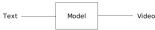
\includegraphics[width=7cm]{multimodality.png}
            \end{center}
    \end{itemize}
\end{frame}

\section{Methodololgy}
\begin{frame}
    
\end{frame}

\section{Experiments}
\begin{frame}
    \frametitle{Experiments} 
    \begin{itemize}
        \item \textbf{Datasets}: MSRVTT, LSMDC, MSVD, DiDeMo.
        \item \textbf{Metrics}: R@K, MdR.
        \item \textbf{Results}:
            \begin{itemize}
                \item MSRVTT
                    \vspace{0.1cm}
                    \begin{center}
                        \includegraphics[width=10cm]{msrvtt.png}
                    \end{center}
            \end{itemize}
    \end{itemize}
\end{frame}

\begin{frame}
    \frametitle{Experiments}
    \begin{itemize}
        \item \textbf{Results}:
    \begin{itemize}
        \item LSMDC
            \begin{center}
                \includegraphics[width=8cm]{lsmdc.png}
            \end{center}
        \item MSVD
            \begin{center}
                \includegraphics[width=8cm]{msvd.png}
            \end{center}
    \end{itemize}
    \end{itemize}
\end{frame}

\begin{frame}
    \frametitle{Experiments}
    \begin{itemize}
        \item \textbf{Results}:
    \begin{itemize}
        \item DiDeMo
            \begin{center}
                \includegraphics[width=8cm]{didemo.png}
            \end{center}
    \end{itemize}
\item \textbf{Ablation studies}.
\item \textbf{Validation of Gaussian assumption}.
    \end{itemize}
\end{frame}

\section{Critical Review}
\begin{frame}
    \frametitle{Critical Review} 
    \begin{itemize}
        \item Readability and structure.
            \begin{itemize}
                \item Illustrate CRET method clearly.
                \item Satisfy requirements of the scientific paper.
            \end{itemize}
        \item Reproducibility: Source code, the availability of data sets, experimental settings.
        \item Importance.
            \begin{itemize}
                \item Theoretical contributions.
                \item Practical applications.
            \end{itemize}
        \item Summary of strong and weak points.
    \end{itemize}
\end{frame}
\end{document}
